\chapter{Vue d'ensemble des notions actuarielles}
\section*{Introduction}
Dans ce chapitre on va parler de la réalisation des estimations ainsi que nos analyses et remarques.
\section{Lecture de données}
Comme indiqué dans l’énoncé on va travailler sur la population danoise bien évidemment notre pays concerné c’est le Danemark. Pour ce faire nous avons eu recours au site Human Mortality Database (HMD). C’est une base de données qui a été créée pour fournir des données détaillées sur la mortalité et la population aux chercheurs, étudiants, journalistes,
analystes des politiques et autres personnes intéressées par l’histoire de la longévité humaine.
on a utilisé la commande hmd.mx()pour le téléchargement. 

\section{Estimation des paramètres d’un modèle de Lee-Carter à partir des données historiques téléchargées}

\begin{figure}[!htb]
 \caption{Taux de mortalité des hommes danois entre 1876 et 2019}
    \centering
    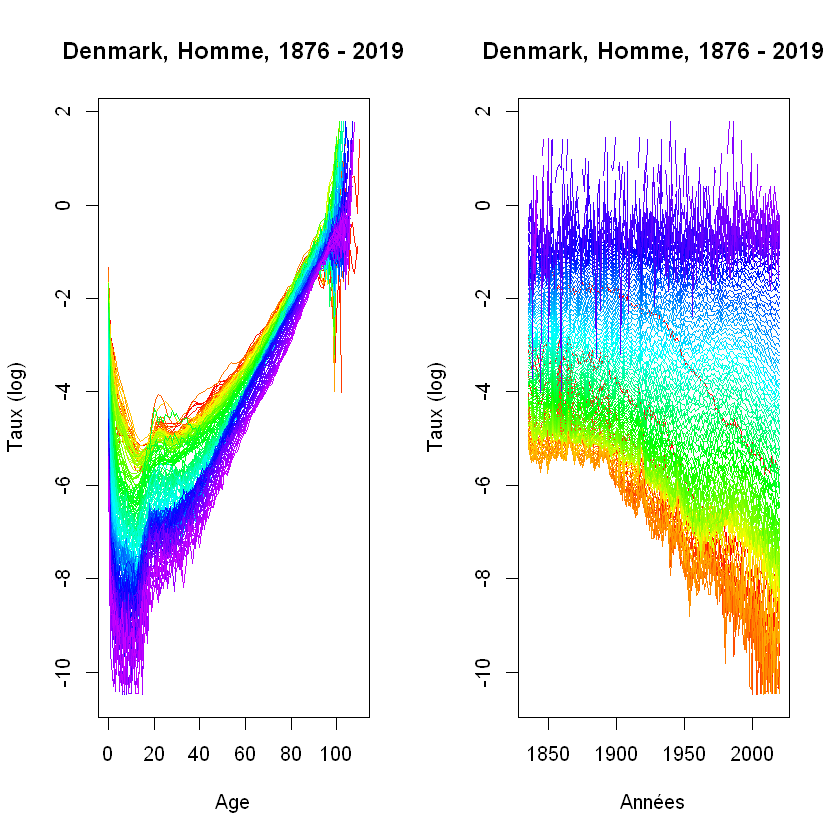
\includegraphics[scale =0.7]{output_7_0.png}
\end{figure}

\begin{figure}[!htb]
 \caption{Taux de mortalité des femmes danois entre 1876 et 2019}
    \centering
    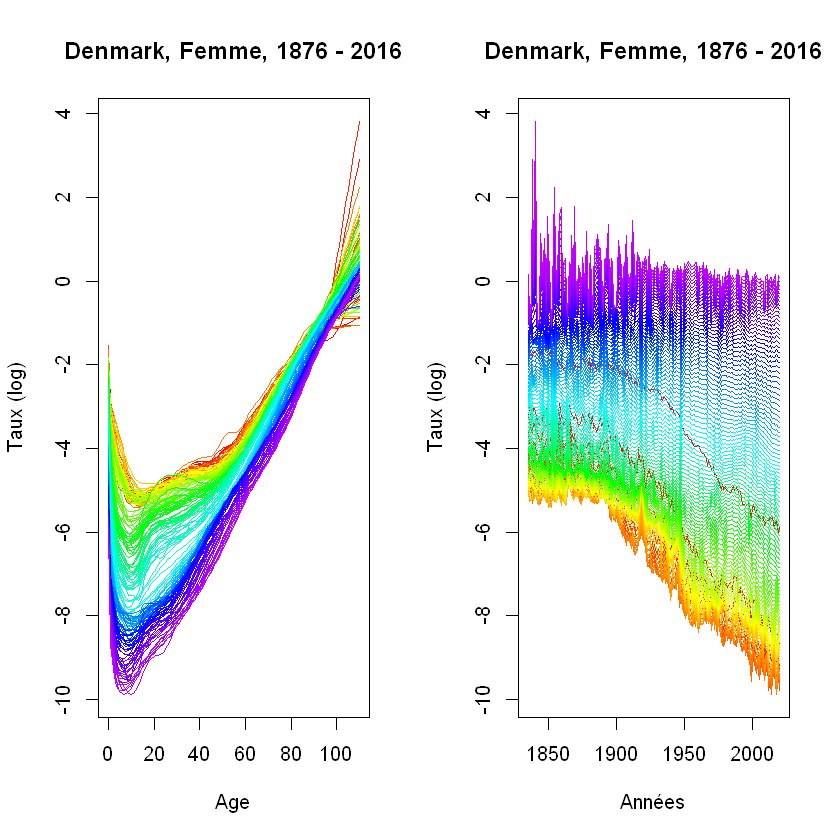
\includegraphics[scale =0.65]{output_7_1.png}
\end{figure}

\begin{figure}[!htb]
 \caption{Danemark, Effets principaux et interactions, Homme 1876-2019}
    \centering
    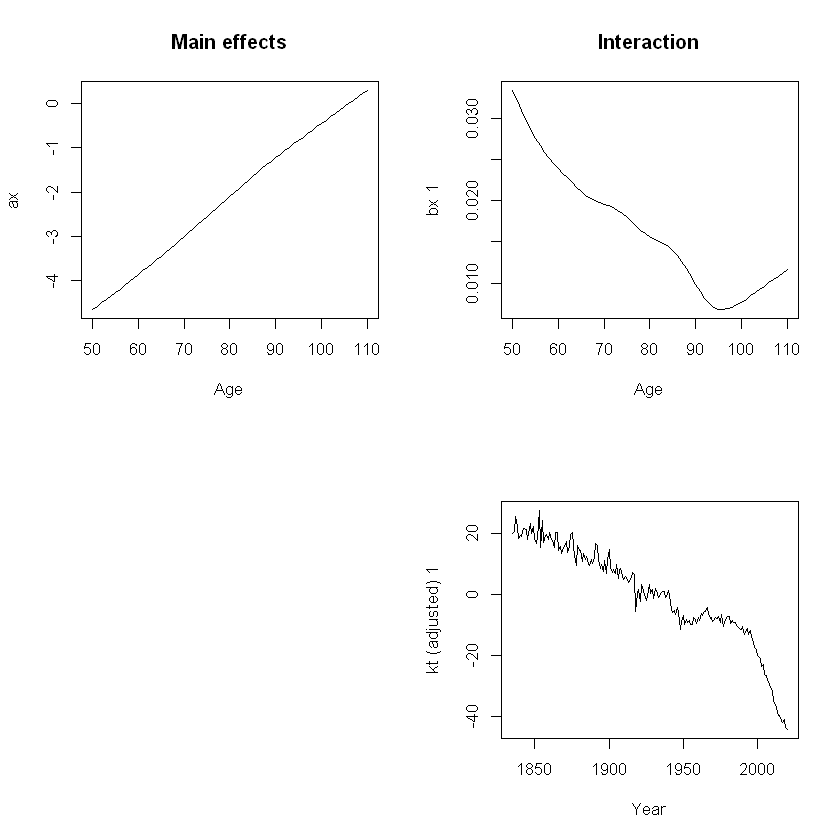
\includegraphics[scale =0.65]{output_7_3.png}
\end{figure}

\begin{figure}[!htb]
 \caption{Danemark, Effets principaux et interactions, Femme 1876-2019}
    \centering
    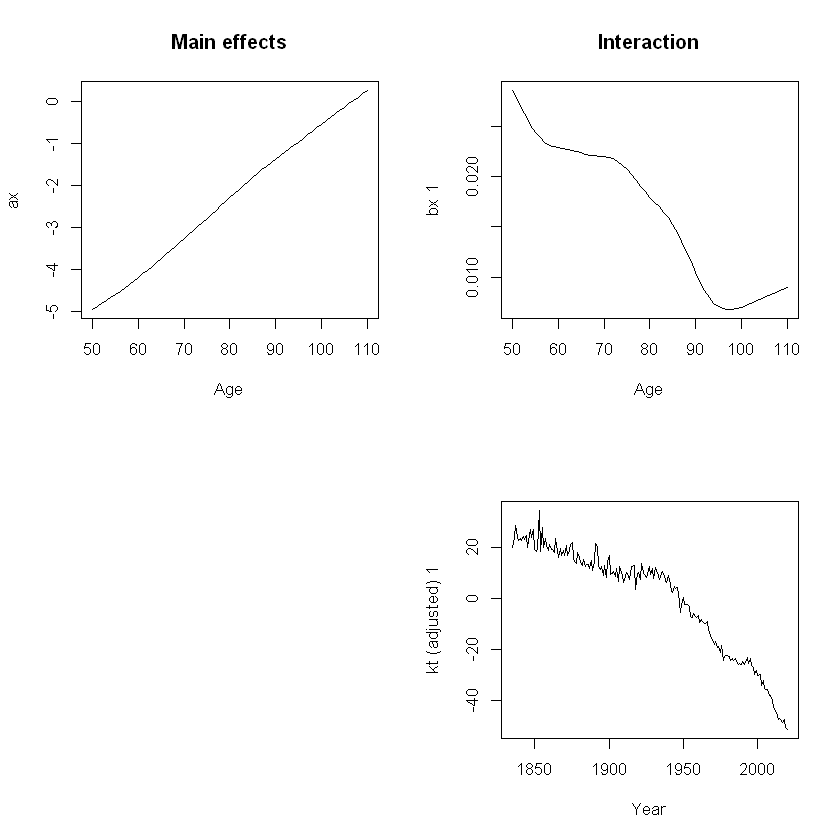
\includegraphics[scale =0.8]{output_7_5.png}
\end{figure}

Analyse des paramètres Pour Femme : ax : la valeur moyenne des logs de la mortalité instantanné ( ln µ(x,t) au cours du temps ) elle crois en fonction de l’age elle varie entre -5 et 0 .

bx indique la sensibilité de la mortalité instantanée par rapport à l’évolution générale de la mortalité. Si on se situe à partir de 55 ans, on constate que les âges les plus sensibles à l’évolution temporelle de la mortalité sont ceux entre 55 et 70 ans . On atteint en effet des stabilités sur ces tranches d’âges.

D’après la figure ci-dessus et comme kt indique l’évolution générale de la mortalité dans le temps ; On constate pendant les années 1860 une forte croissance due à la Seconde guerre du Schleswig qui c'est déroulé pendant la même periode . On constate une tendance linéaire à la décroissance des entre 1940 et 2010 Cette tendance à la décroissance du paramètre k, qui devient négatif au cours de la période, associée à la positivité moyenne du paramètre $\beta$ implique d’après la formule de Lee-Carter, une diminution des taux instantanés de mortalité. En conséquence, on assiste à une augmentation de la probabilité de la survie sur la période observée.

Analyse des paramètres Pour Homme : ax : la valeur moyenne des logs de la mortalité instantanné ( ln µ(x,t) au cours du temps ) elle crois en fonction de l’age elle varie entre -4 et 0 .

bx indique la sensibilité de la mortalité instantanée par rapport à l’évolution générale de la mortalité. on se situe à partir de 55 ans .

D’après la figure ci-dessus et comme kt indique l’évolution générale de la mortalité dans le temps ; On constate pendant les années 1860 une forte croissance due à la Seconde guerre du Schleswig qui c'est déroulé pendant la même periode . On constate une tendance linéaire à la décroissance des entre 1940 et 2010 Cette tendance à la décroissance du paramètre k, qui devient négatif au cours de la période, associée à la positivité moyenne du paramètre $\beta$ implique d’après la formule de Lee-Carter, une diminution des taux instantanés de mortalité. En conséquence, on assiste à une augmentation de la probabilité de la survie sur la période observée.

\begin{figure}[!htb]
 \caption{Le résidus du modèle LCA Pour Homme}
    \centering
    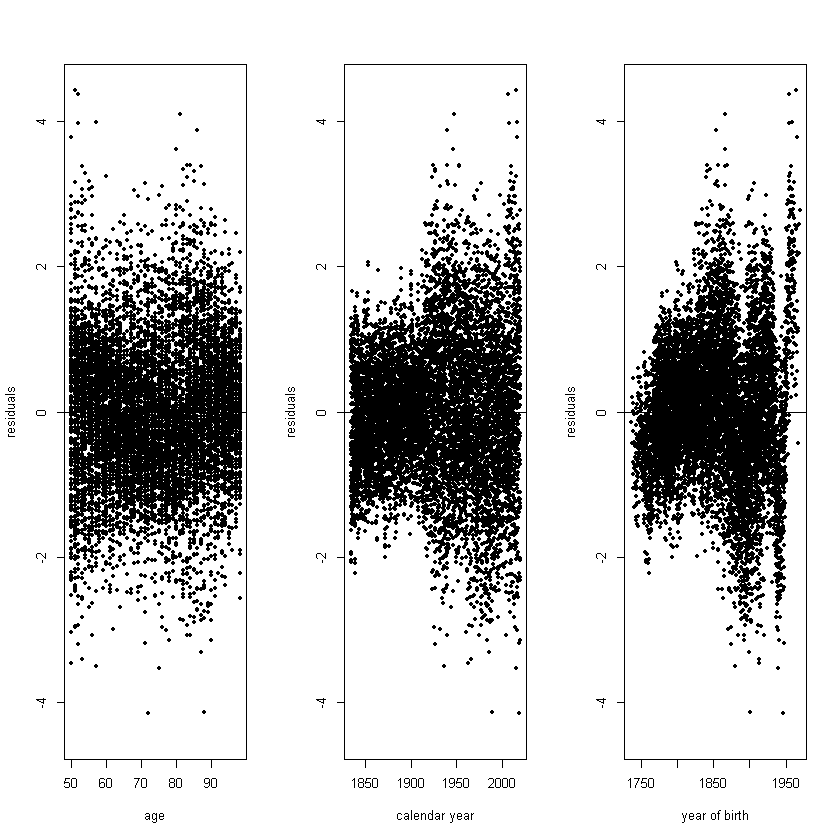
\includegraphics[scale =0.9]{output_9_1.png}
\end{figure}

\begin{figure}[!htb]
 \caption{Le résidus du modèle LCA Pour Femme}
    \centering
    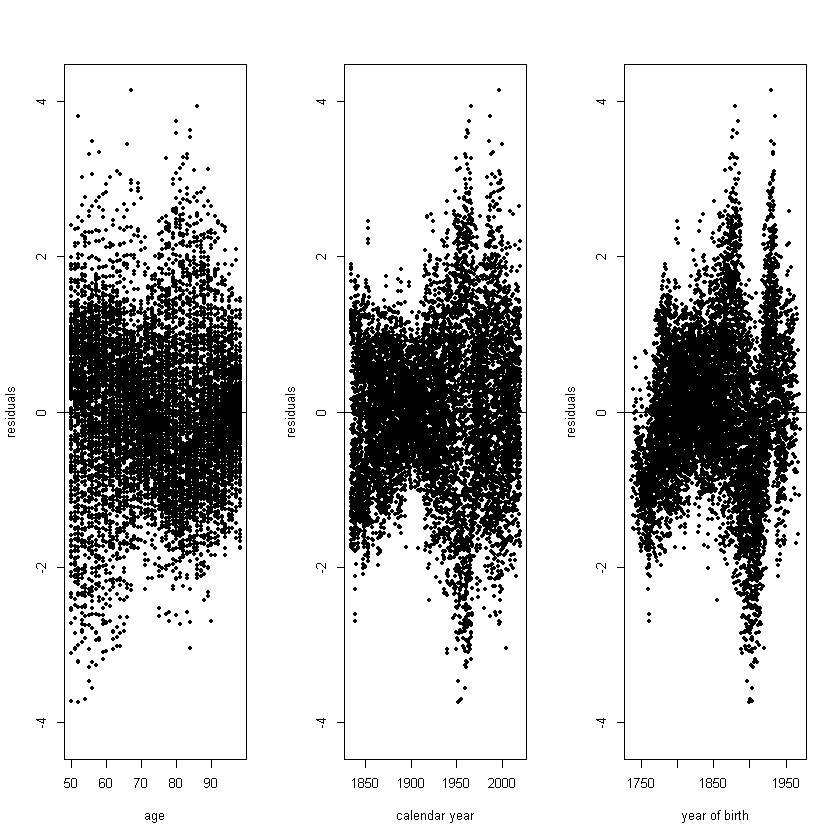
\includegraphics[scale =0.55]{output_11_0.png}
\end{figure}

lorsque l’on effectue un ajustement par la méthode de Lee-Carter, on peut analyser la variance des résidus, et confronter les observations à l’hypothèse d’homoscédasticité.

\section{Estimation des paramètres du modèle de CBD à partir des données historiques téléchargées} 
\begin{figure}[!htb]
 \caption{Danemark, modèle principal de CBD, homme de 50 à 98 ans}
    \centering
    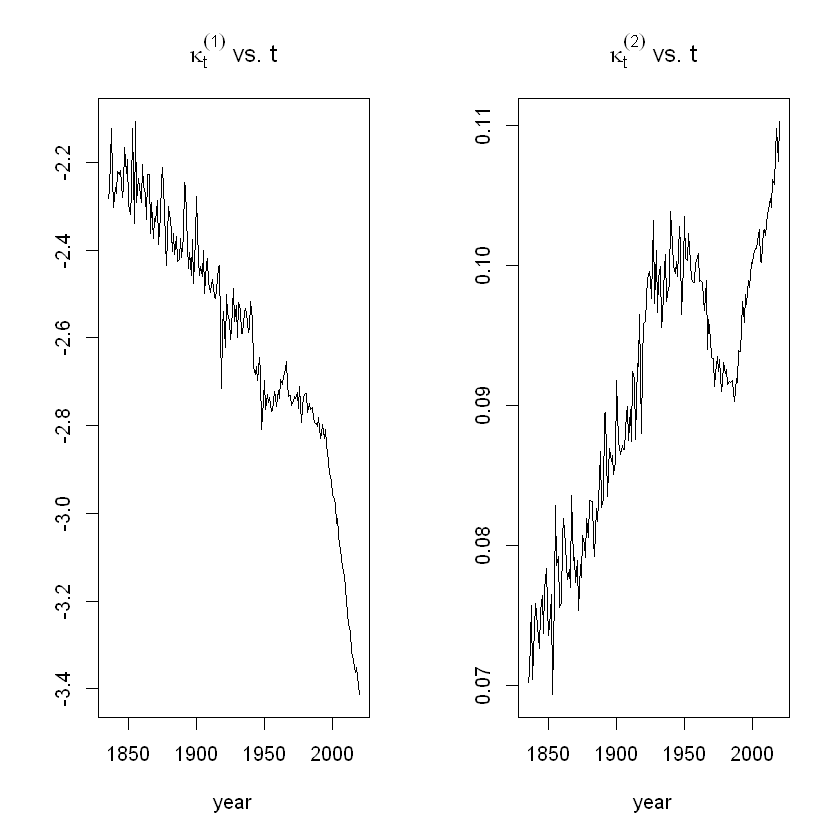
\includegraphics[scale =0.5]{output_18_7.png}
\end{figure}

\begin{figure}[!htb]
 \caption{Danemark, modèle principal de CBD, femme de 50 à 98 ans}
    \centering
    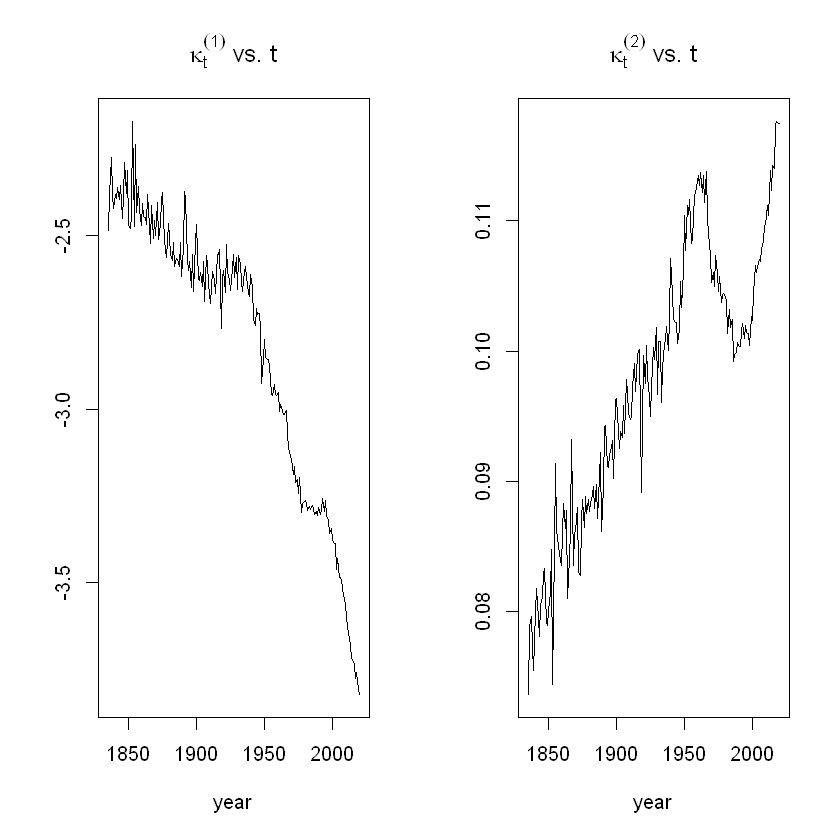
\includegraphics[scale =0.6]{output_18_9.png}
\end{figure}

\section{Log taux de mortalité estimés par le modèle Lee-Carter} 
\begin{figure}[!htb]
 \caption{log taux de mortalité (Danemark, 2010)}
    \centering
    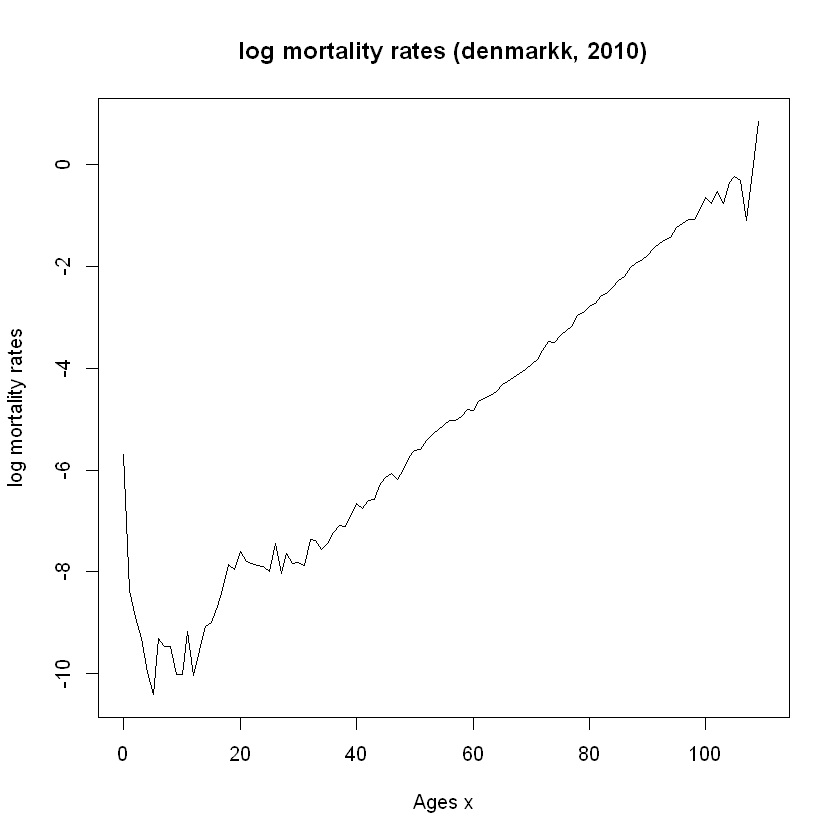
\includegraphics[scale =0.6]{output_20_0.png}
\end{figure}

\section{Procédure par défaut de projection des taux mortalité implémentée dans StMoMo}
Dans la famille des modèles de mortalité stochastique généralisés par âge, période et cohorte, la dynamique de la mortalité est les indices de période kt (i), i = 1, ..., N et l’indice de cohorte yt x. Par conséquent, les prévisions et la simulation des taux de mortalité nécessite la modélisation de ces indices à l’aide de séries chronologiques techniques. Pour les indices de période, nous envisageons deux approches de modélisation alternatives. Une première possibilité est d’utiliser l’approche standard dans la documentation actuarielle et de supposer que les indices de période suivent une multivariée marche aléatoire avec dérive.

\section{Projection des taux de mortalité à l’aide de la fonction forecast}
\begin{figure}[!htb]
 \caption{projection de taux de mortalité Danemark, homme sur 25 ans avec LCA}
    \centering
    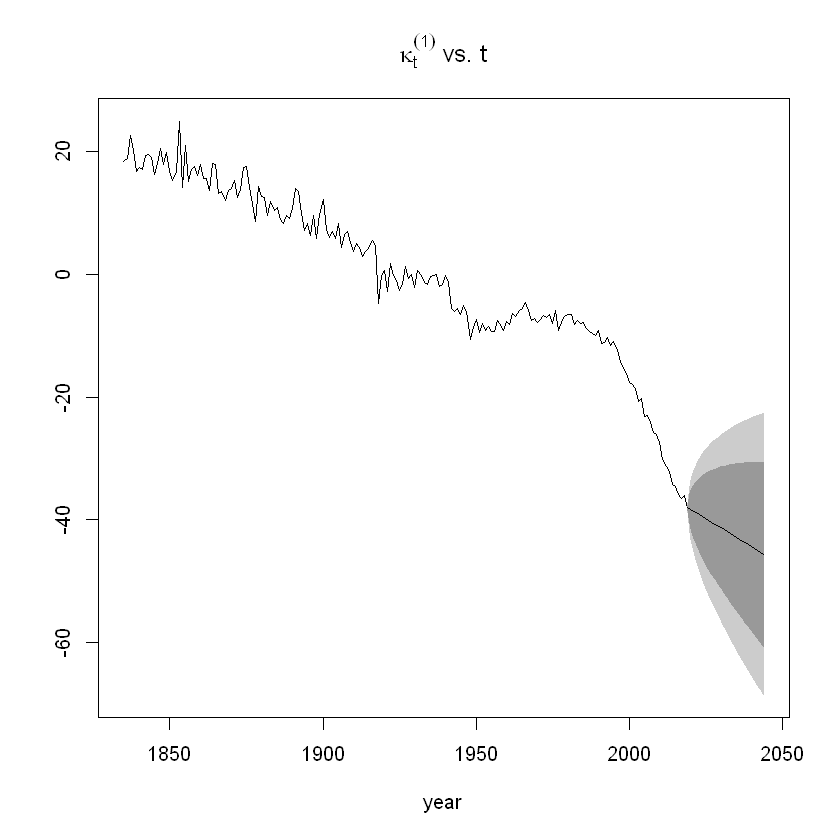
\includegraphics[scale =0.8]{output_24_1.png}
\end{figure}

\begin{figure}[!htb]
 \caption{projection de taux de mortalité Danemark, femme sur 25 ans avec LCA}
    \centering
    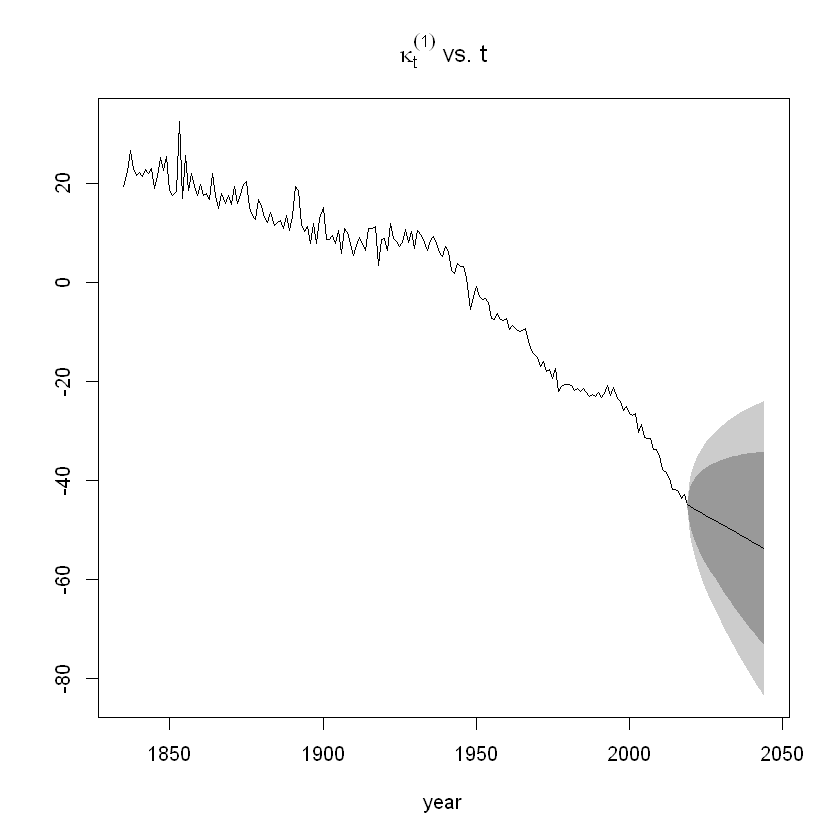
\includegraphics[scale =0.65]{output_24_2.png}
\end{figure}

\begin{figure}[!htb]
 \caption{projection de taux de mortalité Danemark, homme sur 25 ans avec CBD}
    \centering
    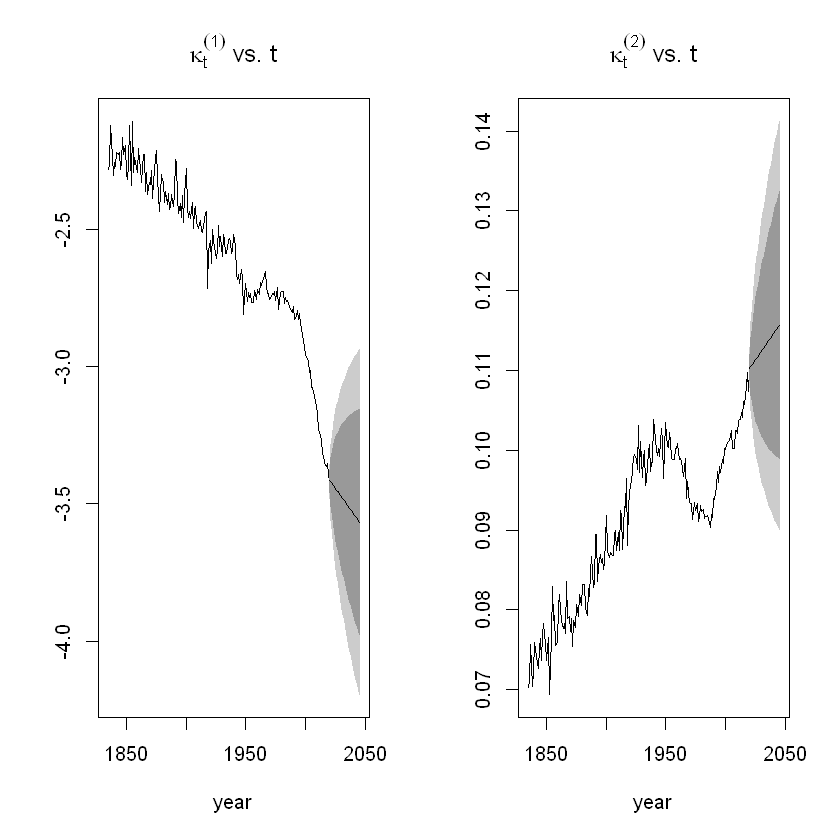
\includegraphics[scale =0.65]{output_25_0.png}
\end{figure}

\begin{figure}[!htb]
 \caption{projection de taux de mortalité Danemark, femme sur 25 ans avec CBD}
    \centering
    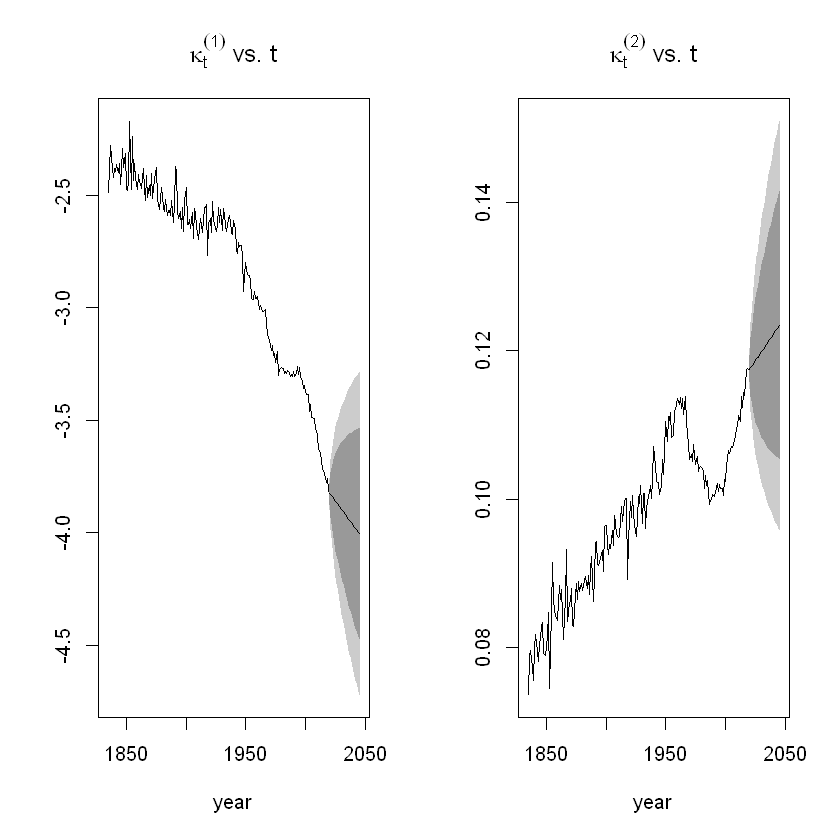
\includegraphics[scale =0.8]{output_25_1.png}
\end{figure}